%*****************************************
\chapter{Ausblick}\label{ch:futurework}
%*****************************************
Möglichkeiten zur Verbesserung der Leistung von Sprachmodellen auf die hier vorgestellten Ziele bieten sich in vielerlei Hinsicht.
Eine Auswahl der erfolgsversprechensten Ansätze wird in diesem Kapitel vorgestellt.

\section{Modellvergrößerung}
Die intuitivste Lösung ist die Vergrößerung der verwendeten Modelle.
Von dem verwendeten Llama 2 Modell gibt es auch Modelle mit 13 Milliarden und 70 Milliarden Parametern.
Bereits im Artikel \citet{llama} über Llama 1 Modelle erreicht nur das größte Modell eine vergleichbare Leistung wie ChatGPT. Es ist also davon auszugehen, dass auch hier größere Modelle eine bessere Leistung erzielen können.
\citet{scaling_laws} haben gezeigt, dass die Leistung eines Modells neben der Größe des Datensatzes und der Länge des Trainings auch von der Größe des Modells abhängt.
Dies unterstützt die hier vorgestellte These.\\

Allerdings bringt eine Vergrößerung des Modells auch Nachteile und Probleme mit sich.
Größere Modelle benötigen mehr Rechenleistung und \ac{gpu}-\ac{ram} während des Trainings und der Inferenz.
Dies führt zu höheren Kosten und längeren Trainingszeiten
und schränkt die Verwendbarkeit der Modelle nach dem Training deutlich ein.
In der hier verwendeten Konfiguration konnte die Anzahl der verwendeten \acp{gpu} nicht erhöht werden,
daher war ein Training größerer Modelle nicht möglich.\\

Größere Modelle neigen schneller dazu, einen Zustand der Überanpassung zu erreichen, weshalb das Training mit einer deutlich geringeren Lernrate durchgeführt wird, was die Trainingszeit weiter erhöht.\\

\subsection{Training durch Quantisierung}
\begin{figure}
    \centering
    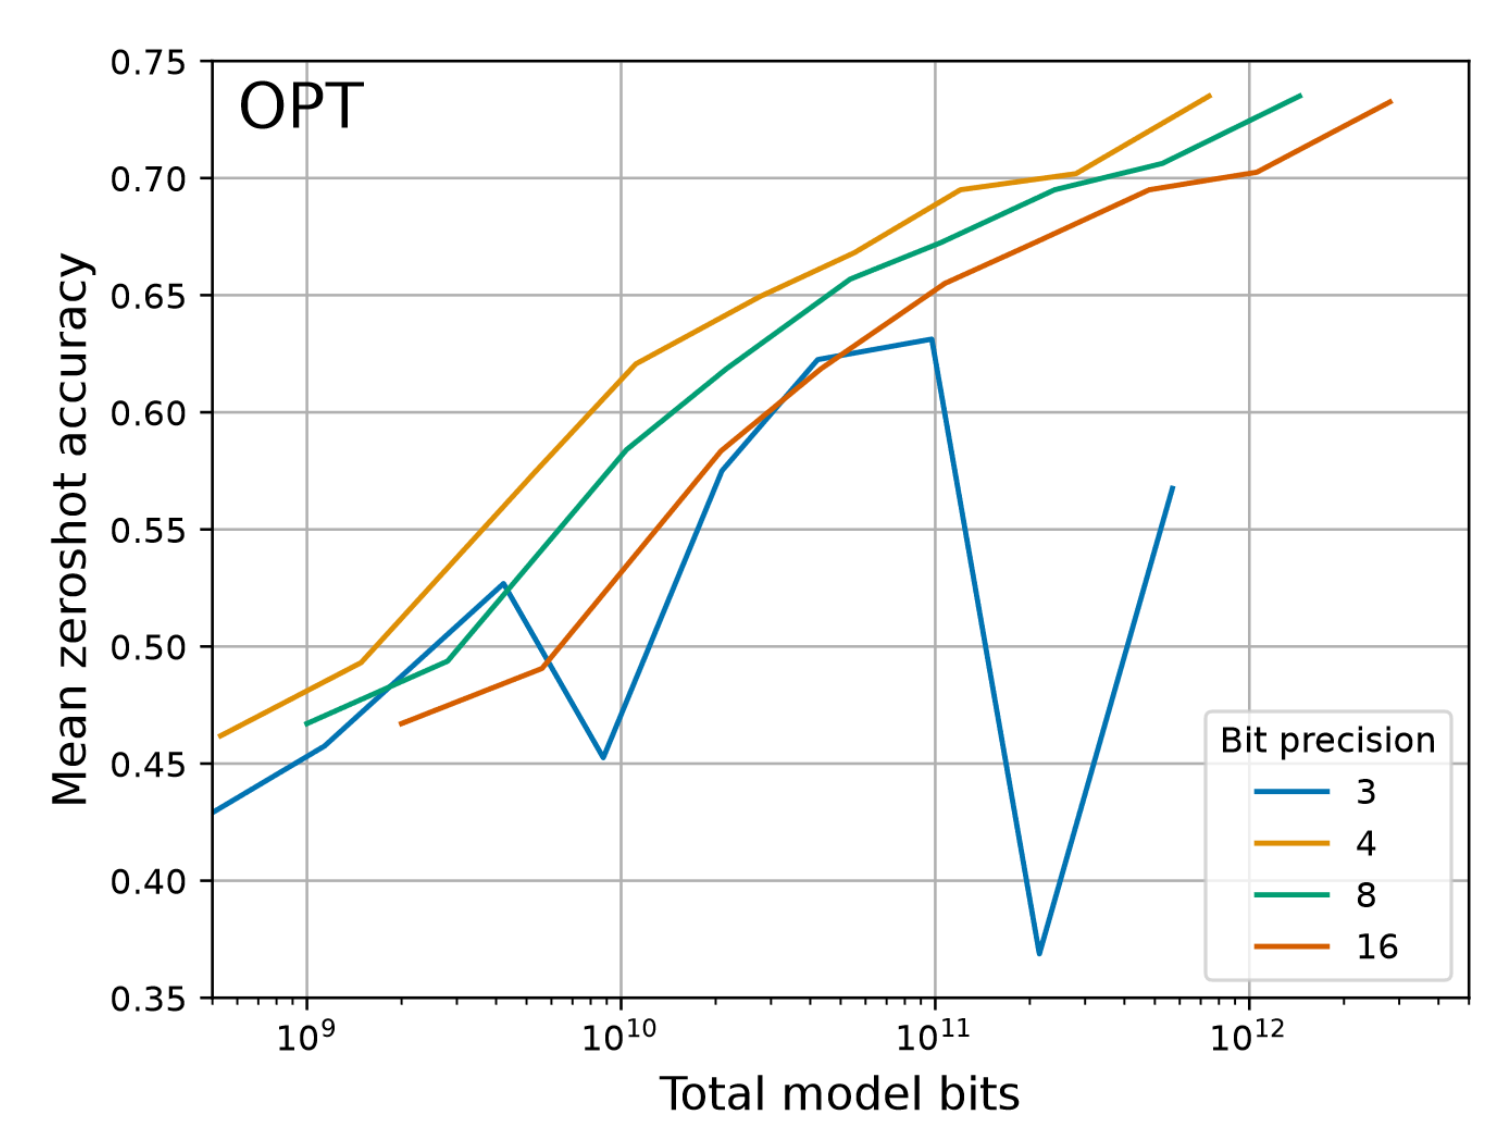
\includegraphics[width=\textwidth]{results/bit_scaling_laws.png}
    \caption[Korrektheit von OPT Modellen nach Modellbits]{Korrektheit von OPT Modellen aufgeteilt nach unterschiedlicher Bitanzahl pro Parameter aus \citet{4bit}. Modelle mit gleicher Parameteranzahl liegen ungefähr auf gleicher X-Achse, jedoch nicht auf gleicher Y-Achse.}%
    \label{fig:bit_scaling}
\end{figure}
Um große Modelle zu trainieren und zu nutzen, ist der Einsatz der \ac{zero}-Optimierung ein erster Schritt, der in \citet{deepspeed} vorgestellt wird.
Mit Hilfe der \ac{zero}-Stufe 3 Optimierung können Optimierungs- und Parameterzustände auf \ac{cpu}s und Festplatten ausgelagert werden, während die Berechnungen weiterhin auf \ac{gpu}s durchgeführt werden.
Zusätzlich kann durch eine Quantisierung der Modelle in kleinere Datentypen die Anzahl der benötigten \ac{gpu}-\ac{ram}s deutlich reduziert werden.
\citet{4bit} untersuchte den Einfluss der Quantisierung auf die Performance der Modelle und zeigte, dass eine Quantisierung auf 4 Bit die Leistung der Modelle nur geringfügig beeinflusst.
\cref{fig:bit_scaling} zeigt die Korrektheit von OPT-Modellen mit unterschiedlichen Datentypen (3, 4, 8 und 16 Bit).
Modelle mit gleicher Parameteranzahl liegen nicht auf dem gleichen Y-Achse, da die X-Achse in Modellbits angegeben ist.
Modelle mit der gleichen Anzahl von Parametern, aber einer geringeren Anzahl von Bits pro Parameter sind daher weiter links in der Grafik angeordnet.
Dennoch zeigen diese Abbildung von \citet{4bit} und ähnliche Abbildungen für andere Modelltypen eine fast identische Leistung bis einschließlich 4 Bit.\\

Zusätzlich ist es möglich, Modelle während der Inferenz in einen 8-Bit-Modus zu konvertieren, um Ressourcen zu sparen.
\citet{8bit-inference} haben gezeigt, dass bei der Verwendung von 8-Bit-Matrix-Multiplikationen keine signifikanten Leistungseinbußen zu erwarten sind.
Der 8-Bit Inferenzmodus wurde auch in dieser Arbeit verwendet, um die trainierten Modelle auf einer Nvidia Tesla A30 GPU mit \SI{24}{\giga\byte} \ac{ram} nutzen zu können.\\

\section{Human Reinforcement Learning}
Nach erfolgreichem Training eines Modells kann dessen Ausgabe wesentlich verbessert werden, indem Menschen die Ausgabe bewerten und das Modell entsprechend anpassen.
Dieser Schritt wurde auch bei GPT4 durchgeführt und ist einer der Gründe für die hohe Leistungsfähigkeit des Modells.
Mit Hilfe des so genannten Human Reinforcement Learning können Modelle darauf trainiert werden, Erklärungen zu ihren Antworten zu geben, unbeantwortete Fragen mit z.B. der generierten Antwort \enquote{Ich weiß es nicht} zu markieren, auf schädliche Inhalte nicht zu reagieren oder die Antwort zu verweigern und Texte klarer und freundlicher zu formulieren.
Dieser Trainingsschritt ist jedoch sehr aufwendig und kann nicht vollständig automatisiert werden.\\

Llama 2 verfügt über Versionen, die dieses Human Reinforcement Learning bereits durchlaufen haben.
In dieser Arbeit wird davon ausgegangen, dass dieses zusätzlich erlernte Wissen verloren geht, sobald ein Continual Pretraining durchgeführt wird.
Diese Annahme basiert auf der Tatsache, dass populäre Modelle das Human Reinforcement Learning als letzten Trainingsschritt durchlaufen haben.
Eine Widerlegung dieser Hypothese könnte potenziell auch die Leistung der Modelle verbessern.

\section{Datensatzvergrößerung}
Eine wesentliche Einschränkung der hier trainierten Modelle ist die Größe des Trainingsdatensatzes.
Mit etwa \num{34500} Tokens ist dieser Datensatz nicht mit den für das ursprüngliche Training verwendeten Datensätzen vergleichbar und erreicht nur eine Größe von \SI{600}{\kilo\byte}. Kleine Datensätze führen zu einer schnelleren Überanpassung, da der Datensatz mehrfach verwendet werden muss, bevor eine Anpassung des Modells an diesen erfolgen kann.
Dies zeigt sich auch in den Ergebnissen, da bereits nach 3 Epochen eine Überanpassung zu erkennen ist.
Größere Datensätze führen zu weniger Epochen und damit zu weniger Überanpassung.
Zudem enthalten größere Datensätze potentiell gleiche Informationen in unterschiedlicher Formulierung, was wiederum die Generalisierbarkeit des Modells verbessert.
Insbesondere die Kriterien Robustheit und Fragenverständnis profitieren von größeren Datensätzen.\\

Für die Verwendung größerer Datensätze wäre es optimal, weitere Literatur zum Thema Informationssysteme im Gesundheitswesen heranzuziehen.
Wichtig ist dabei, dass die Wissensinhalte identisch sind, so dass sich die Aussagen zwischen den Büchern nicht widersprechen.
Auch eine Zusammenstellung einzelner Kapitel aus verschiedenen Quellen mit gleichem Inhalt könnte die Größe des Datensatzes erhöhen und damit die Leistung der Modelle verbessern.\\

\section{Domänenspezifische Modelle}
Das Llama 2 Modell wurde ohne speziellen Fokus auf eine Domäne, insbesondere die Domäne Medizininformatik, trainiert.
Allgemein trainierte Modelle können einen breiteren Anwendungsbereich abdecken, enthalten aber auch weniger Verständnis einzelner Domänen als domänenspezifische Modelle.
Die Verwendung von Modellen, die stärker auf die Domäne der Medizininformatik oder auf wissenschaftliche Inhalte fokussiert sind, könnte die Basisleistung des Modells und damit auch die Endleistung der hier trainierten Modelle verbessern.\\

Leider existieren zum Zeitpunkt dieser Arbeit keine domänenspezifischen Modelle in der Größe von Llama 2, da entweder die Größe der Modelle oder die Größe des Datensatzes geringer ist.
Domänenspezifische Modelle können auch Informationen enthalten, die im Widerspruch zum verwendeten Trainingsdatensatz stehen, aber besser gelernt wurden, weil mehr Informationen im ursprünglichen Datensatz vorhanden waren.
Das bewusste Verlernen dieses falschen Wissens ist nicht trivial und kann die Leistung des Modells negativ beeinflussen.
Eine Möglichkeit der Modellanpassung wurde von \citet{knowledge_neurons} vorgestellt, um bestimmte Wissensneuronen aus einem Modell zu entfernen.

\section{Adapter-basiertes Training}\label{sec:adapter-training}
Wie bereits in \cref{ch:relatedWork} erwähnt, ist neben den klassischen Trainingsmethoden auch das Training mit Hilfe von Adaptern möglich.
\citet{adapterhub} stellt eine Plattform zur Verfügung, die es erlaubt, kleinere Neuronale Netze zwischen die Modellschichten einzufügen und diese zu trainieren.
Dies minimiert die benötigten Ressourcen, verkürzt die Trainingszeit und verhindert das Verlernen von Wissen.
Adapter müssen speziell für Modelltypen entwickelt werden und sind zum Zeitpunkt dieser Arbeit nicht für Llama-Modelle verfügbar.
Eine eigene Implementierung für die Llama Modelle könnte die endgültige Performance der Modelle verbessern.\\

Neben dem Einfügen von Adaptern ist auch die Verwendung von \ac{lora}, eingeführt in \citet{lora}, möglich.
\ac{lora} erlaubt das Einfügen von trainierbaren Matrizen in jede Schicht und hat ähnliche Vorteile wie Adapter.
Die Verwendung von \ac{lora} wurde im Rahmen dieser Arbeit untersucht, jedoch nicht in die endgültige Auswertung übernommen, da eine Inferenz nicht möglich war.

\section{Textextraktion aus Kontext}
Diese Arbeit konzentriert sich primär auf die Verwendung von Decoder-basierten Modellen zur Generierung von Antworten auf Fragen.
Grund dafür ist die potentiell höhere Generalisierbarkeit auf Formulierungen um besser generierten Text zu erhalten.
Neben der Generierung von Text ist auch die Extraktion von Text aus einem gegebenen Kontext eine mögliche Lösung.
Mit Hilfe von Encoder-basierten Modellen wie z.B. \ac{bert} ist es möglich, Textpassagen, die Antworten auf gegebene Fragen enthalten, aus einem Kontext zu extrahieren.
Dieser Ansatz könnte zu einer besseren Korrektheit der Fragen führen, allerdings könnten andere Kriterien wie Robustheit und Erklärbarkeit darunter leiden.\\

\section{Retrieval Augmented Generation}
Man könnte auch ganz auf das Training von Decoder-basierten Modellen verzichten, bei denen das Modell die Frage nur mit Hilfe eines gegebenen Kontextes beantworten soll.
Dieser Ansatz verspricht sehr gute Ergebnisse, da Modelle wie GPT4 bereits sehr gute Leistungen bei der Extraktion von Informationen aus Kontexten zeigen.\\

\citet{context-extract} haben dieses Verhalten an großen Sprachmodellen untersucht und gezeigt, dass Modelle in der Lage sind, Informationen aus Anfang und Ende eines Kontextes weitgehend korrekt zu extrahieren.
Um nur den Kontext zur Beantwortung von Fragen zu verwenden, müssen Modelle mit einer großen Kontextlänge gewählt und das verwendete Buch optional gekürzt werden. \citet{extending-context} beschreibt eine Möglichkeit, die verfügbare Kontextlänge mit Hilfe von positionsabhängiger Interpolation zu erweitern.\\
Eine Kombination aus einem Encoder-basierten Modell zur Bestimmung der Textposition und einem Decoder-basierten Modell zur Generierung einer Antwort mit Hilfe der extrahierten Textposition könnte ebenfalls Abhilfe schaffen. Dieser Ansatz wurde von \citet{retrieval-1} untersucht und erzielte \ac{sota} Ergebnisse in drei \ac{qa} Evaluationsdatensätzen. Ähnliche Ergebnisse wurden von \citet{retrieval-2} in ihrem Artikel erreicht.\\

Dieser Ansatz erfordert kein weiteres Training von Modellen und führt dementsprechend zu deutlich weniger Leistungsanforderungen. Das bedeutet, dass größere Modelle unter gleicher Hardware genutzt werden können und damit auch die erwarteten Ergebnisse höher ausfallen könnten. Die Komplexität liegt hierbei in der Integration der Modelle zu einem Gesamtsystem und der Veränderung bereits existierender Modelle um größere Kontextlängen zu ermöglichen.

\section{Zusammenfassung}
Die hier vorgestellten Richtungen für zukünftige Arbeiten versprechen eine Verbesserung der Leistung der Modelle in vielerlei Hinsicht.
Zum besseren Überblick stell \cref{tab:future-work} eine Übersicht über die hier vorgestellten Ansätze dar.
Die Tabelle ist nach Erfolgseinschätzung sortiert.
Ein hoher Aufwand bedeutet grundlegende strukturelle Änderungen im genutzten Prozess und erfordert dementsprechend hohen Zeit- und Kostenaufwand.

\begin{table}
    \centering
    \resizebox{\textwidth}{!}{%
    \begin{tabular}{lll}
        \toprule
        \textbf{Ansatz}                   & \textbf{Aufwand} & \textbf{Erfolgseinschätzung}             \\
        \midrule
        Retrieval Augmented Generation    & hoch                                          & sehr hoch \\
        Datensatzvergrößerung             & niedrig                                       & hoch      \\
        Modellvergrößerung                & hoch                                          & hoch      \\
        Human Reinforcement Learning      & sehr hoch                                     & hoch      \\
        Domänenspezifische Modelle        & niedrig                                       & mittel    \\
        Textextraktion aus Kontext        & niedrig                                       & mittel    \\
        Adapter-basiertes Training        & mittel                                        & mittel    \\
    \end{tabular}}
    \caption[Verbesserungsansätze der Modelle]{Übersicht über mögliche Ansätze zur Verbesserung der Leistung der Modelle}\label{tab:future-work}
\end{table}
